\section{Virtual Private Networks}

\subsection{Introduction to VPNs}

\begin{definition}{Virtual Private Network (VPN)}\\
A VPN is a private network created within a public network infrastructure:
\begin{itemize}
    \item \textbf{Private} - External parties cannot read or modify transmitted data
    \item \textbf{Virtual} - Privacy is achieved through cryptography, not dedicated links
    \item Creates an encrypted tunnel between endpoints
    \item Allows secure access to resources across untrusted networks
\end{itemize}
\end{definition}

\begin{concept}{VPN Use Cases}\\
Common VPN use cases include:
\begin{itemize}
    \item Connecting remote offices or branches to a main corporate network
    \item Allowing partner organizations limited access to internal resources
    \item Enabling remote employees to securely access company resources
    \item Protecting privacy when using public Wi-Fi networks
    \item Bypassing geographical restrictions on content
\end{itemize}
\end{concept}

\begin{theorem}{VPN Core Concepts}\\
Key VPN characteristics include:
\begin{itemize}
    \item VPNs connect networks (or a host to a network), not just individual hosts
    \item VPN endpoints (gateways) establish and maintain the secure tunnel
    \item Internal hosts typically require no special configuration
    \item Traffic is encrypted between VPN endpoints
    \item VPNs often hide internal addressing with NAT
\end{itemize}
\end{theorem}

\subsection{VPN Protocols}

\begin{definition}{VPN Protocol Types}\\
Several protocols are commonly used to implement VPNs:
\begin{itemize}
    \item \textbf{IPsec} - IP Security protocol suite operating at the network layer
    \item \textbf{OpenVPN} - SSL/TLS-based solution running at the application layer
    \item \textbf{WireGuard} - Modern, high-performance VPN protocol
    \item \textbf{Proprietary protocols} - Vendor-specific implementations
\end{itemize}
\end{definition}

\subsection{IPsec VPNs}

\begin{concept}{IPsec Components}\\
IPsec consists of several components:
\begin{itemize}
    \item \textbf{Authentication Header (AH)} - Provides authentication and integrity (rarely used)
    \item \textbf{Encapsulating Security Payload (ESP)} - Provides encryption, authentication, and integrity
    \item \textbf{Internet Key Exchange (IKE)} - Handles key exchange and security association negotiation
    \item \textbf{Security Associations (SA)} - Parameters for secure communication
\end{itemize}

ESP provides confidentiality, authentication, and integrity protection for IP packets. It operates at the network layer and can protect entire IP packets in tunnel mode or just the payload in transport mode.

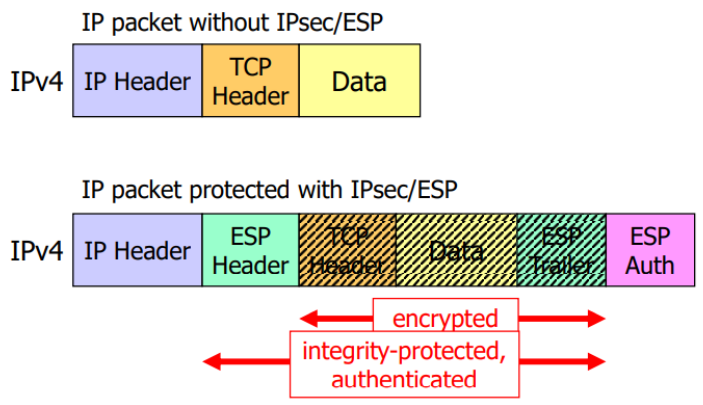
\includegraphics[width=\linewidth]{IPsec.png}

Sequence numbers in IPsec are used to order packets and drop duplicates, providing replay protection:

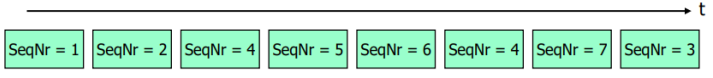
\includegraphics[width=\linewidth]{IPsec_sequence_nr.png}
\end{concept}

\begin{theorem}{IPsec vs. TLS Comparison}\\
IPsec and TLS differ in several key aspects:
\begin{itemize}
    \item \textbf{Layer} - IPsec works at the network layer, TLS at the transport/application layer
    \item \textbf{Protection scope} - IPsec protects all IP traffic between hosts, TLS protects specific application connections
    \item \textbf{Implementation} - IPsec requires kernel integration, TLS runs in user space
    \item \textbf{Configuration} - IPsec typically requires more complex configuration
\end{itemize}
\end{theorem}

\begin{concept}{IPsec Modes}\\
IPsec operates in two primary modes:
\begin{itemize}
    \item \textbf{Transport Mode}:
    \begin{itemize}
        \item Protects the payload of the IP packet
        \item Original IP header remains intact
        \item Typically used for host-to-host communications
    \end{itemize}
    \item \textbf{Tunnel Mode}:
    \begin{itemize}
        \item Protects the entire original IP packet
        \item Encapsulates the original packet in a new IP packet
        \item Typically used for network-to-network (gateway-to-gateway) VPNs
        \item Hides internal IP addressing from eavesdroppers
    \end{itemize}
\end{itemize}
\end{concept}


\subsection{OpenVPN}

\begin{concept}{OpenVPN Architecture}\\
OpenVPN's architecture includes several key components:
\begin{itemize}
    \item \textbf{Virtual network interfaces} (TUN/TAP) to capture and inject network traffic
    \item \textbf{SSL/TLS library} for authentication and key exchange
    \item \textbf{Control channel} for management communication
    \item \textbf{Data channel} for encrypted user traffic
    \item \textbf{Configuration system} for defining connection parameters
\end{itemize}
\end{concept}

\begin{theorem}{OpenVPN Protocol Features}\\
OpenVPN offers several protocol features:
\begin{itemize}
    \item Can operate over UDP (default, port 1194) or TCP
    \item Uses SSL/TLS for authentication and key exchange
    \item Implements reliability mechanisms when using UDP
    \item Employs OpenSSL for cryptographic operations
    \item Supports various authentication methods:
    \begin{itemize}
        \item Pre-shared static keys
        \item Certificate-based authentication
        \item Username/password authentication
        \item Multi-factor authentication
    \end{itemize}
\end{itemize}
\end{theorem}

\subsection{WireGuard}

\begin{concept}{WireGuard Architecture}
WireGuard's architecture focuses on simplicity:
\begin{itemize}
    \item Operates at the network layer (Layer 3)
    \item Implements a "cryptokey routing" concept
    \item Uses public key authentication
    \item Always employs perfect forward secrecy
    \item Maintains a simple, stateless design
\end{itemize}
\end{concept}

\begin{theorem}{WireGuard Features}
Key features of WireGuard include:
\begin{itemize}
    \item \textbf{Simplified cryptography} - No cipher negotiation, uses fixed set of modern algorithms
    \item \textbf{Fast handshake} - 1-RTT handshake under normal circumstances
    \item \textbf{Clean, minimal codebase} - Easier to audit and more secure
    \item \textbf{Connection-less design} - No persistent connection state
    \item \textbf{Stealth operation} - No response to unauthenticated packets
    \item \textbf{DoS mitigation} - Cookie challenge mechanism
    \item \textbf{Seamless roaming} - Maintains connections across network changes
\end{itemize}
\end{theorem}


\subsection{Comparing VPN Protocols}

\begin{concept}{Protocol Comparison}
IPsec, OpenVPN, and WireGuard have different characteristics:
\begin{itemize}
    \item \textbf{IPsec}:
    \begin{itemize}
        \item Pro: Widely supported, mature standard
        \item Pro: Hardware acceleration in many devices
        \item Con: Complex implementation and configuration
        \item Con: May be blocked by restrictive firewalls
    \end{itemize}
    \item \textbf{OpenVPN}:
    \begin{itemize}
        \item Pro: Cross-platform compatibility
        \item Pro: Runs in user space
        \item Pro: Works well through firewalls (can use TCP port 443)
        \item Con: Slower performance than IPsec and WireGuard
    \end{itemize}
    \item \textbf{WireGuard}:
    \begin{itemize}
        \item Pro: Superior performance and simplicity
        \item Pro: Modern cryptography by default
        \item Pro: Small, auditable codebase
        \item Con: Less mature than alternatives
        \item Con: Fixed cryptographic algorithms
    \end{itemize}
\end{itemize}
\end{concept}

\subsection{VPN Deployment Scenarios}

\begin{concept}{Site-to-Site VPN}
Site-to-site VPNs connect entire networks:
\begin{itemize}
    \item Connect branch offices to headquarters
    \item Connect partner organizations' networks
    \item Implemented using VPN gateways at each location
    \item Transparent to end users
    \item Typically always-on connections
\end{itemize}
\end{concept}

\begin{concept}{Remote Access VPN}
Remote access VPNs connect individual users to a network:
\begin{itemize}
    \item Enable employees to work remotely
    \item Allow access to internal resources from outside
    \item Implemented using VPN client software on user devices
    \item Often use dynamic IP addressing with virtual addresses
    \item Typically on-demand connections
\end{itemize}
\end{concept}
